\documentclass{beamer}
\usepackage{amsmath}
\usepackage{amsfonts}
\usepackage{amssymb}
\usepackage{polski}
\usepackage{pgfplots}
\pgfplotsset{compat=1.15}
\usepackage{mathrsfs}
\usetikzlibrary{arrows}
\usetheme{Warsaw}
\usefonttheme[onlymath]{serif}
\usepackage{animate}
\usepackage{caption}
\usepackage{graphicx}

\title{Być albo nie być czarną dziurą}
\author[F. Hansdorfer \and J. Winiarczyk \and Ł. Parda
\and T. Gruss]{Franciszek Hansdorfer \and Jacek Winiarczyk \and Łukasz Parda
\and Tomasz Gruss\\{\small Opiekun projektu: dr hab. Radosław Poleski}}
\date{\today}

\begin{document}

\begin{frame}
    \titlepage
\end{frame}

\section{Wprowadzenie do soczewkowania grawitacyjnego}
\subsection{Soczewkowanie grawitacyjne}

\begin{frame}
    \begin{columns}
        \begin{column}{0.5\linewidth}
            \begin{itemize}
                \item Ogólna teoria względności $\implies$
                \item Masa zakrzywia czasoprzestrzeń $\implies$
                \item Światło idące w pobliżu masy jest odchylane $\implies$
                \item Obserwator widzi obiekty za zakrzywiającą masą w inny sposób $\implies$
                \item Soczewkowanie grawitacyjne
            \end{itemize}
        \end{column}
        \begin{column}{0.5\linewidth}
            \begin{figure}
                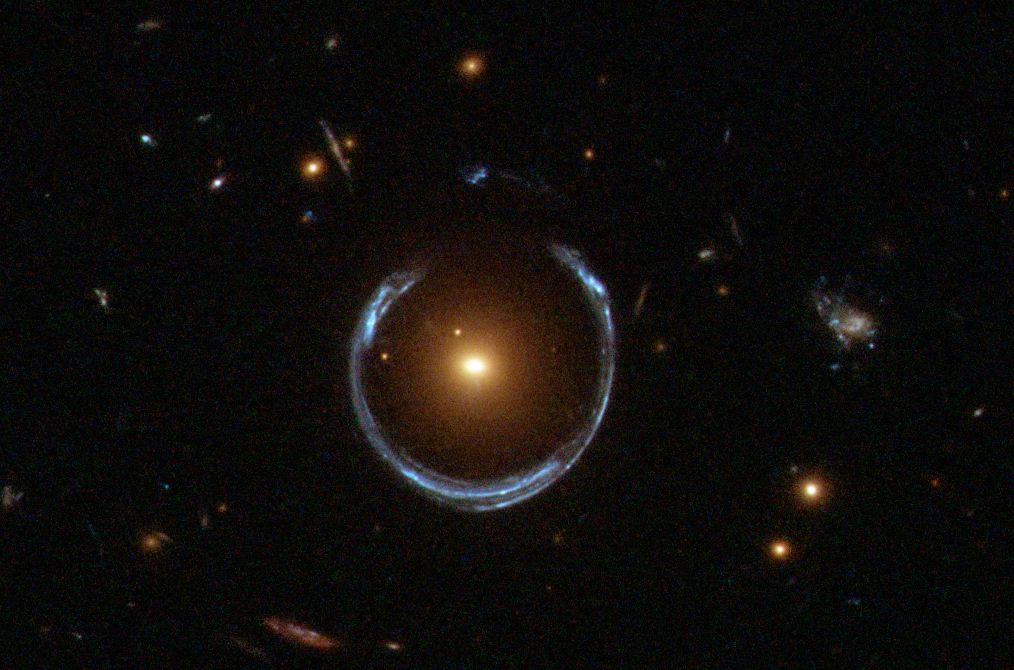
\includegraphics[width=\textwidth]{A_Horseshoe_Einstein_Ring_from_Hubble.jpeg}
                \caption*{\tiny{ESA/Hubble, NASA}}
            \end{figure}
        \end{column}
    \end{columns}
\end{frame}

\begin{frame}
    \begin{figure}
        \centering
        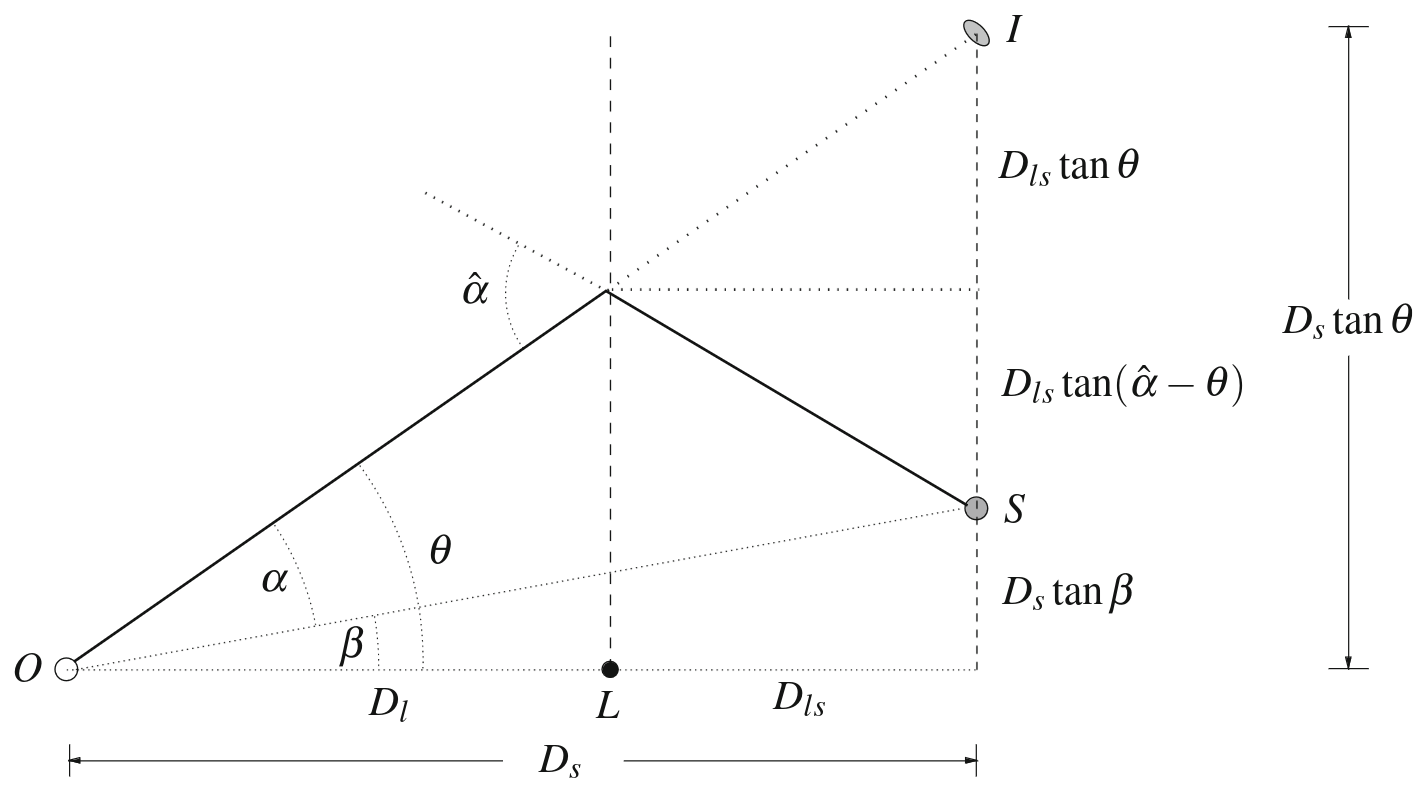
\includegraphics[width=0.6\textwidth]{Screenshot from 2024-06-10 13-41-41.png}
        \caption*{\tiny{Principles of Gravitational
                Lensing, Arthur B. Congdon, Charles R. Keeton}}
    \end{figure}
    \textbf{Równanie soczewki}:
    \[\beta = \theta - \alpha(\theta)\]

\end{frame}

\begin{frame}
    \textbf{Równanie soczewki}:
    \[\beta = \theta - \alpha(\theta)\]
    Dla punktowej masy mamy:
    \[\alpha(\theta) = \frac{4GM}{c^2\theta}\frac{D_s-D_l}{D_s D_l}\]
    \[\theta_E = \sqrt{\frac{4GM}{c^2}\frac{D_s-D_l}{D_s D_l}}\]
    Wtedy:
    \[\beta = \theta - \frac{4GM}{c^2}\frac{D_s-D_l}{D_s D_l}\frac{1}{\theta}\]

\end{frame}

\subsection{Mikrosoczewkowanie}
\begin{frame}{Mikrosoczewkowanie}
    \begin{columns}
        \begin{column}{0.6\linewidth}
            \[M \sim M_{\odot}\]
            Na przykład dla $D_s = 8 \text{ kpc}$, $D_l = 4 \text{ kpc}$, $M = 1 M_{\odot}$:
            \[\theta_E = 0.32 \text{ mas}\]
            Dla $u = \frac{\beta}{\theta_E}$ wzmocnienie źródła określa wzór:
            \[A(u) = \frac{u^2 + 2}{u \sqrt{u^2 + 4}}\]
            $u$ możemy natomiast obliczyć znając $u_0, t_0, t_E$:
            \[u(t) = \sqrt{u_0^2 + \left(\frac{t-t_0}{t_E}\right)^2}\]
        \end{column}
        \begin{column}{0.4\linewidth}
            \begin{figure}
                \centering
                \animategraphics[width =\textwidth, loop, autoplay]{24}{animation1/Scott_Gaudi_anim-}{0}{65}
                \caption*{\tiny{Animation by B.S. Gaudi - microlensing-source.org}}
            \end{figure}
        \end{column}
    \end{columns}

\end{frame}

\subsection{Odchylenia od modelu punktowego źródła i soczewki}

\section{Modelowanie soczewkowania}
\subsubsection{MulensModel}

\section{Rezultaty}

\end{document}